\documentclass[11pt,a4paper]{article}
\usepackage[T1]{fontenc} \usepackage{lmodern} \usepackage[utf8]{inputenc} \usepackage[english]{babel} \usepackage{amssymb} \usepackage{amsmath} \usepackage[round]{natbib} \usepackage{xcolor,graphicx}
\author{Billy Afablulatur} \title{A simple proof of last Fermat’s theorem} \date{\today}
\begin{document}
\maketitle

\section{Introduction}
\subsection{section{test and citation example}
Hello World. Mister Resnick wrote a beautiful book about Harry, see \citep{Resnick92}. If you want something more fancy, try \citet{Baddeley07}.
\\By looking at the plot we cannot definitely exclude that there might exist some seasonal patterns. To detect if a seasonality effect is really present in the series, we test it by modelling the seasonality and add it in the linear model. 
\section{section}
(summary coefficients)
We can see that none of the estimated seasonal coefficients are significant. Therefore we only need to eliminate the trend. In the absence of a seasonal component our model becomes the following (Brook Davis p. 24):
\begin{equation}
X_t = m_t + Y_t, \text{t = 1,...,n,} 
\\where EY_t = 0
\end{equation} 

In order to construct a model for our data (with no seasonality) we try first to fit a polynomial trend by least squares. We fit a linear trend, a quadratic trend aswell as a logarithmic trend in order to handle a potential exponential increase in rents, even though at first sight the trend (figure xy) looks more likely linear than exponential. 
\subsection{subsection}
We can see that the coefficients in all 3 models are highly significant and with an $R^2$-Value of 0.98 both, the linear and the quadratic model explain our data extremely well. The logarithmic model shows a bit less explanatory power with an $R^2$-Value of 0.72 but anyhow its coefficient is aswell highly significant. However we have to be careful with the interpretation of the p-values since this regression models assume independancy of the observations whereas our goal is different, meaning to use regression in order to construct a stationary timeseries (Brooks Davis p. xy).


Unfortunately the plots for polynomial trend elimination are not stationary as we can see in figure x-y. They are large covariances and it looks that the are evidentally depending on time $t$ therefore they are non-stationary. Furthermore/in addition all three graphs have a lot of significant lags which  doesn't die out quickly, so we can conclude our covariances depend on time and therefore the series is non-stationary. The Ljung-Box test examines whether there is significant evidence for non-zero correlations at lags 1-40. Small p-values (i.e., less than 0.05) suggest that the series is stationary. The Augmented Dickie-Fuller test and the Kwiatkowski-Phillips-Schmidt-Shin (KPSS) test provide strong evidence that these three series fitted by polynomial trends are non-stationary. Even though we have to keep in mind the low power of Dickie-Fuller Test for our purposes given the fact this test assumes a AR-Process, about which we cannot be sure.

Since we cannot get stationary residuals by fitting polynomial trends we have to use different methods. Hence, we try to remove the trend from the data by differencing the data at different lags (1,2 and 4) in order to generate a noise sequence and therefore get a stationary series (brook davis p.35). The following three figures show the differenced series derived from the quarterly rents for lag = 1, 2 and 4.

For all three models we were able to generate stationary residuals which don't depend on time. However figure (lag1) shows mostly patterns of a white noise. This white-noise patterns is aswell indicated by the sample autocorrelation function (FIgure xy) for lag1-differencing where all lags upt to 40 fall well within the bounds of $+/-1.96sqrt{98}$ (brooks davis p.39). The Ljung-Box-Test (Ljung-Box 1978, see brooks davis p. 36) indicates a p-value of 0.35, meaning that we cannot reject the iid-Hypothesis $H_0$ that there is independence between the observations. Therefore The Ljung-Box-Test emphasizes furthermore the independence of the values and the white-noise-patterns of the lag-1-differencing-method. Since White-Noise would mean E0 and Variance sigma no more modelling would be necessary. In order to get better predictions and forecasting than by white-noise-residuals we try the model for lag2 differencing, since an iid noise model for the resiudals apprears to be inappropriate for the lag2-differencing, indicating by the ACF with shows at least correlation at lag1 and some other lags are touching the $+/-1.96sqrt{98}$ - bounds. Furthermore/in addition the diff-lag2-graph has a few significant lags but these die out quickly, so we can conclude our series is stationary.
Cross-validation with a test data set considering only the last 35 of the 100 observations confirms furthermore the non-stationary character of the lag-2-differencing-model 
Box.test(d2.indiceloyers.test, lag=2, type="Ljung-Box") p-value of 0.033 suggests the data are (time-)independent
adf.test(d2.indiceloyers.test, alternative = "stationary", k=2)  H0 of non-stationarity cannot be rejected which is not a problem, that could be due to lack of observations
kpss.test(d2.indiceloyers.test)  with a p-value>0.05 the test data seems to be stationary aswell
the data of the training and the test data set (from 2009 Q4 to 2018 Q1) are independent, however we can see a slight increase in the training data set indicating that in the years from 1993 to 2009 the growth in rental prices was higher than in the years in the test data set which begins after 2009. that can be explained by the big baisse in the early 90ies, starting from a lower initial point and better conjunctural perspectives the increase was stronger, whilst from 2009 on the growth in rental prices slowed down, which can be very well explained by the US subprime crises beginning in the year 2008 and the following global recession.

Differencing by lag4 is not appropriate neither since there is too much autocorrelation showed by the ACF a lot of bars outside the $+/-1.96sqrt{98}$ - bounds.

from L6/7 p. 25. 
From the visualization of the sample ACF and sample PACF we can guess an AR(1) model as a suitable model for our data, since the ACF-plot shows only the first bar outside the borders (besides the following three touching them which we consider to give us to less evidence to justify an AR-model with of order more than 1.
our sample PACF ahat (h) is significantly different than zero for all h smaller or equal than 2 and becomes negligible for h larger than 2. indicating that a suitable model for the could be p=2 so an AR(2) rpocess. . This is further emphasized by the plot where the sample PACF values beyond lag 2 are approximately i.i.d. with a N(0,1/n) distribution. Therefore in our supposed AR(2) process rouglhly 95 percent of the sample PACF values beyond lag 2 should be within the bound +/- 1.96/sqrt(n) which is in fact true according to the plot (no single bar after p=2 is outside the bound +/-1.96/sqrt(n). sample PACF satisfyise |alpha(h)|>1.96/sqrt(n) for h<=p and |alpha(h)| < 1.06/sqrt(n) for h>p, which suggest an AR(p=2) model for our data.
in other words: The fact that all of the PACF values beyond lag 3 fall within the bounds suggests the possible suitability of an AR(p=3) model for the mean corrected data set Xt=St-46.93. One simple way to estimate the parameters phi1 phi2 phi33 and sigma2 of such a model is to require tha the ACVF of the model at lags 0,1 and 2 should match the sample ACVF at those lags. Substituting the sample ACVF vlaues gammahat0 gammahat1 gammahat2 for gammma0 gamma1 and gamma 2 in the first thee equations of (3.2.5) and (3.2.6) and solving for phi1 phi2 phi3 and sigma2 gives the fitted model Xt-1.318xt-1+255Xtte-2+sxt-3=Zt wit hZt  WN (this method of model fitting is called yule-walker estimation ) (brock davis p. 99)

Furthermore the choice of an AR(p) model is underlined by the fact that the ACF pot shows an exponentially decreasing patterns of |rho(h)| and PACF patterns with p=3 "spikes". Exponentially decrease in AR and alpha(h)=0 for h>p=3 in PACF are typical properties for an AR(p)-process.

In addition to the visualised evidence provided above further analytical evidence for an AR(1)-process is provided by the preliminary prediction by using the Yule-Walker-Algorithm for estimating roughly the AR-coefficients (phi). As we can see in table xy only the first estimated coefficient is a strong coefficient, all the others are close to zero and therefore not significant, emphasizing our assumption to go on with an AR(1)-Model.
The program used from the ITSMR pakage will search thorugh all the Yule-Walker AR(p) models, p=0,1,....,27, selecting the one with smallest AICC value. (explain AICC, corrected AIC) The minimum-AICC Yule-Walker AR model turns out to be the one defined by (eq 5.1.14) with p=1 and AICC value 74.541

In addition the estimated coefficient by Yule-Walker-Algorithm guarantees us that our model is causal. We can see that aswell in table x which shows indicating that the unit root is (slightly) outside the unit circle, with an value of 1.023714.

causality of a process (brock davis p. 85)

HannanRissanen-Algoritm shows strongly varying coefficients theta (q) for different fixed numbers of coefficients
which further underlines our assumption that an AR(p)-model suits our data well instead of an MA(q) or ARMA(p,q) process.


BrockwellDavis p. 193 a root near 1 of the autoregressive polynomial suggests that the data should be differenced before fitting an AMA model, whereas a root near 1 of the moving-average polynomial indicates that the data were overdifferenced. 

\begin{figure}
\centering
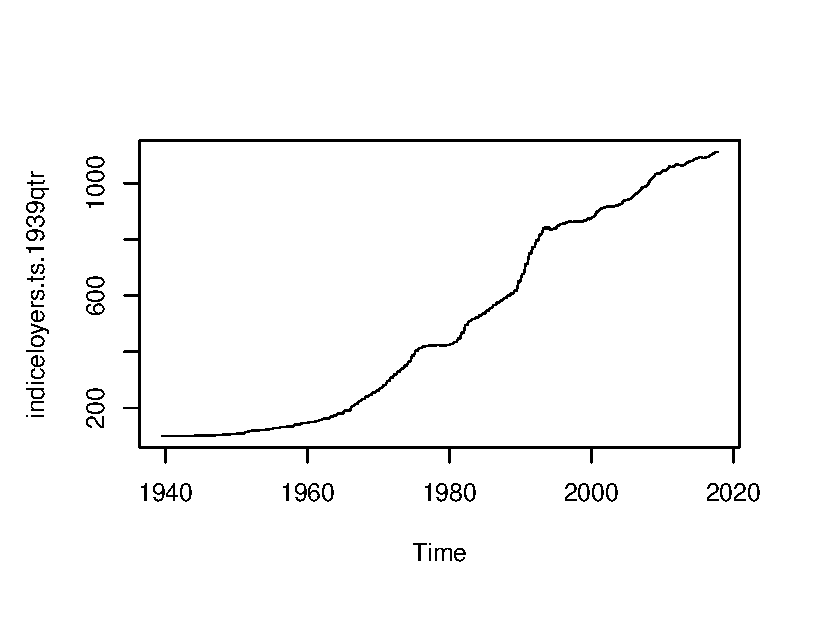
\includegraphics[angle=0,
width=0.5\textwidth]{plot_1939quarterly}
\caption{This is a test.}
\end{figure}
\bibliography{Bibliography}
\bibliographystyle{apa}
\end{document} 
